% 学部生向け説明スライド: 逆回しの数学 — 可逆計算と2枚の鏡
% ビルド: latexmk -lualatex intro-slides.tex
\documentclass[aspectratio=169,11pt]{beamer}
\usepackage{luatexja}
\usepackage{luatexja-fontspec}
\usetheme{metropolis}
\setbeamertemplate{navigation symbols}{}
\usepackage{amsmath,amssymb}
\usepackage{booktabs}
\usepackage{tikz}
\usetikzlibrary{arrows.meta,positioning}

\title{逆回しの数学}
\subtitle{可逆計算・2枚の鏡・60年前の未解決問題}
\author{横山研究室}
\date{2026年度 卒研テーマ紹介}

\begin{document}

\begin{frame}
  \titlepage
\end{frame}

\begin{frame}{計算は「逆回し」できるか}
  \begin{itemize}
    \item ふつうのプログラムは情報を捨てる。\(x \mathrel{:=} 0\) と書いた瞬間、元の \(x\) は消える
    \item \alert{可逆計算}は捨てない計算。実行をビデオの逆再生のように巻き戻せる
    \item なぜ研究する？
    \begin{itemize}
      \item 物理の原理（情報を消すと必ず熱が出る --- Landauer）
      \item 量子計算の回路はすべて可逆
      \item デバッグ・undo・データ圧縮の理論的な土台
    \end{itemize}
  \end{itemize}
\end{frame}

\begin{frame}{今日の主役: 「2回やると元に戻る」関数}
  \begin{block}{対合（involution）}
    \(f(f(x)) = x\) がすべての \(x\) で成り立つ関数
  \end{block}
  \begin{itemize}
    \item 例: 符号反転 \(x \mapsto -x\)、ネガポジ反転、大文字と小文字の交換
    \item 暗号機エニグマも対合（暗号化と復号が同じ操作）
    \item 中野圭さん（Nakano, RC 2020）の発見:
    \begin{itemize}
      \item \alert{機械の設計図が左右対称}な Turing 機械（ITM）を定義すると、
        計算できる関数がちょうど「計算可能な対合」全体になる
      \item 意味（\(f^2 = \mathrm{id}\)）と形（遷移表の対称性）がぴったり一致する、珍しくて美しい定理
    \end{itemize}
  \end{itemize}
\end{frame}

\begin{frame}{自然な次の問い}
  \begin{center}
    {\Large 「2回で戻る」ができたなら、「3回で戻る」は？「\(n\) 回」は？}
  \end{center}
  \vspace{1em}
  \begin{itemize}
    \item 素朴なアイデア: 機械に \(\mathbb{Z}/3\) の対称性を入れればよい？
    \item \alert{失敗する}。2 が特別なのは「実行の逆再生」という操作が位数 2 だから。
      「3分の1だけ逆再生」に対応する機械操作は存在しない
    \item ここで発想の転換 ↓
  \end{itemize}
  \begin{block}{二対合分解定理（本プロジェクト、Lean で機械証明済み）}
    \(n\) 回で元に戻る計算可能な関数は、必ず
    \(f = \iota_1 \circ \iota_2\)（計算可能な対合2つの合成）に分解できる
  \end{block}
\end{frame}

\begin{frame}{証明のこころ: 回転は2枚の鏡でつくれる}
  \begin{columns}
    \begin{column}{0.55\textwidth}
      \begin{itemize}
        \item 正 \(n\) 角形の回転は、2本の鏡映軸での反射の合成
        \item 万華鏡・ダンスの「振り付けの逆再生」と同じ原理
        \item 関数の各軌道（ぐるぐる回る点の輪）ごとに
          「折り返し」を2つ用意すればよい
        \item 中学生に説明できる絵が、計算可能性の世界でもそのまま通用する
      \end{itemize}
    \end{column}
    \begin{column}{0.4\textwidth}
      \centering
      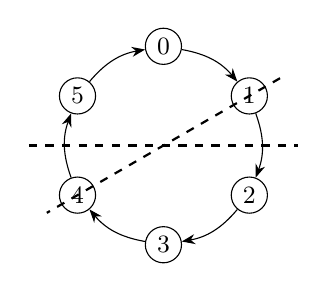
\begin{tikzpicture}[scale=0.9]
        \foreach \i in {0,...,5} {
          \node[circle,draw,inner sep=2pt] (v\i) at ({90-\i*60}:1.4) {\small \i};
        }
        \foreach \i [evaluate=\i as \j using {int(mod(\i+1,6))}] in {0,...,5} {
          \draw[-{Stealth}] (v\i) to[bend left=20] (v\j);
        }
        \draw[dashed,thick] (-1.9,0) -- (1.9,0);
        \draw[dashed,thick] ({30}:1.9) -- ({210}:1.9);
      \end{tikzpicture}

      \small 回転 = 鏡 \(\times\) 鏡
    \end{column}
  \end{columns}
\end{frame}

\begin{frame}{どこまで分解できる？ --- 境界線の発見}
  \begin{itemize}
    \item 軌道が有限なら: いつでも分解できる（軌道を一周して端から折り返す）
    \item 軌道が無限の鎖（\(\ldots \to -1 \to 0 \to 1 \to \ldots\)）だと:
      折り返しには\alert{中心}が要るが、無限の鎖のどこが中心かを
      \alert{アルゴリズムで選べない}ことがある
  \end{itemize}
  \begin{block}{境界定理（本プロジェクト）}
    軌道の全体像がアルゴリズムで見渡せる（軌道所属が決定可能な）置換は、
    すべて2つの計算可能な対合の積に書ける
  \end{block}
  \begin{itemize}
    \item では見渡せないときは？ --- ここから先が今年の冒険だった
  \end{itemize}
\end{frame}

\begin{frame}{60年の系譜と、届いた1通の複写}
  \begin{itemize}
    \item この問題系は Kent (1962) → \alert{Higman (1990, 遺作)} → Boege (2016) と
      細く続く系譜がある
    \item Higman の論文は電子版が存在せず、
      \alert{図書館の文献複写（ILL）でカナダの大学から取り寄せた}
    \item 届いた22ページを読むと:
    \begin{itemize}
      \item p.143 に「\(\rho\) が \(\rho^{-1}\) と共役かどうか、私には分からない」
        --- 我々が立てた予想は\alert{Higman 本人が残した未解決問題}だった
      \item さらに読み進めると、彼の第2の構成が我々の主予想を
        \alert{すでに解決していた}ことも判明（文献には明示されていなかった）
    \end{itemize}
    \item 教訓: 原典を読む。アブストラクトと孫引きでは研究はできない
  \end{itemize}
\end{frame}

\begin{frame}{今年確定した「結果の地図」}
  \begin{center}
  \begin{tabular}{ll}
    \toprule
    置換のタイプ & 2つの対合に分解できる？ \\
    \midrule
    軌道がぜんぶ有限 & \alert{必ずできる}（Lean 証明済み） \\
    軌道が決定可能 & \alert{必ずできる} \\
    Higman の第2構成 & \alert{絶対にできない}（何と合成しても不可） \\
    横断集合が免疫（病的） & \alert{どちらもありうる}（鏡映複製 vs 統合構成） \\
    \bottomrule
  \end{tabular}
  \end{center}
  \vspace{0.5em}
  \begin{itemize}
    \item 分解の可否を決めるのは軌道の「複雑さ」ではなく、
      鎖どうしの\alert{大域的な鏡映対称性}の有無
    \item 特徴づけ定理: 分解できる \(\iff\) 軌道への作用が対合になる
      計算可能な逆転写像を持つ（半シフト補正の技法）
  \end{itemize}
\end{frame}

\begin{frame}{おまけの冒険: 反射のコストを測る}
  \begin{itemize}
    \item 分解 \(\iota_2\) の値を1個計算するのに、\(f\) を何回呼ぶ必要がある？
    \item ゲームとして定式化し、コンピュータで\alert{厳密に全数計算}
    \item 最初の測定（小さいサイズ）から法則 \(\lceil(\ell-1)/2\rceil\) を予想
      → \alert{間違いだった}
    \item 最適戦略の中身をソルバから取り出して解読すると、真の法則は
      \[ q = \min(\ell - 2,\; k_1^{*})\qquad(\text{約数の算術がジャンプを決める}) \]
    \item Lean の \texttt{native\_decide} で小さいケースを機械証明し、
      2つの独立実装の突き合わせで証明のバグも1つ検出・修正
  \end{itemize}
  \begin{center}
    \small 数表を眺めるだけでは足りない。戦略を読み、実装を2つ書き、機械に検証させる
  \end{center}
\end{frame}

\begin{frame}{この研究のやり方（きみが使う道具）}
  \begin{columns}
    \begin{column}{0.5\textwidth}
      \textbf{実験}
      \begin{itemize}
        \item Python で小さい実例を全数計算
        \item 最適戦略・反例の自動探索
      \end{itemize}
      \textbf{証明}
      \begin{itemize}
        \item 紙とペン（敵対者論法・優先度法）
        \item Lean 4 + mathlib で機械証明
      \end{itemize}
    \end{column}
    \begin{column}{0.5\textwidth}
      \textbf{文献}
      \begin{itemize}
        \item Semantic Scholar / Crossref で裏取り
        \item 必要なら ILL で原典を取り寄せる
      \end{itemize}
      \textbf{公開}
      \begin{itemize}
        \item すべて GitHub で公開しながら進める
        \item \texttt{github.com/yokoyama-lab/periodic-tm}
      \end{itemize}
    \end{column}
  \end{columns}
\end{frame}

\begin{frame}{卒研テーマ（とっかかり付きで待っています）}
  \begin{itemize}
    \item \textbf{★ シミュレータと可視化} --- 動く最小実装あり。
      逆再生が「1歩通り過ぎる」現象の修正から始められる
    \item \textbf{★★ 分解のコスト解析} --- ベンチマークあり。
      実測 \(2n\) 回/評価の上界証明から
    \item \textbf{★★ Bennett 可逆化の Lean 機械化} --- 演習5問（模範解答つき）から
    \item \textbf{★★★ 未解決問題} --- 位数 \(n\) をネイティブに実現する機械モデル。
      いまは「存在しない」方向の証明を追っている
  \end{itemize}
  \vspace{0.5em}
  \begin{center}
    各テーマの README・演習・実装 → \texttt{periodic-tm/themes/}
  \end{center}
\end{frame}

\begin{frame}{まとめ}
  \begin{itemize}
    \item 「2回で戻る」機械（ITM）から出発し、
      「\(n\) 回で戻る」計算の世界を2枚の鏡で分解した
    \item 分解の境界線は「軌道を見渡せるか」「鏡映対称性があるか」で決まる
    \item 60年前の系譜に接続し、Higman の未解決問題に部分回答を与えた
    \item 実験 → 予想 → 反証 → 解読 → 証明 → 機械検証、のサイクルを
      全部 GitHub 上で公開しながら回した
  \end{itemize}
  \vspace{1em}
  \begin{center}
    {\large 枯れた数学を土台に、新しい問いの境界線を自分の手で引く。\\
    興味があれば \texttt{themes/} をのぞいてください。}
  \end{center}
\end{frame}

\end{document}
